\documentclass{article}
\usepackage[preprint]{neurips_2025}
\usepackage[utf8]{inputenc}
\usepackage[T1]{fontenc}
\usepackage{hyperref}
\usepackage{url}
\usepackage{booktabs}
\usepackage{amsmath}
\usepackage{graphicx}
\usepackage{microtype}
\usepackage{xcolor}
\usepackage{tabularx}

\title{Evolving Chart-QA Inference for a 2B Vision-Language Model:\\
An AlphaEvolve-Style System, Manual Baselines, and an Honest Holdout}

\author{Ahmadreza Farvardin}

\begin{document}
\maketitle

\begin{abstract}
We build an AlphaEvolve-style evolution system that uses an LLM to rewrite the \texttt{vlm\_inference} function of
Qwen3-VL-2B-Instruct and Qwen3-VL-2B-Thinking for the descriptive questions of CharXiv, and compare it with our own
manual optimization. On an 800-query holdout split that no design decision used, manual tuning lifts the naive
Instruct baseline from 25.9\,\% to 56.0\,\% while making it 6$\times$ faster; evolution adds a further
\textbf{+6.0 points} (62.0\,\%, McNemar $p=0.0003$) at the same speed, and makes the Thinking model
\textbf{33\,\% faster and 2.2 points more accurate} (67.0\,\%, $p=0.01$). The most accurate system is the evolved
Thinking model (67.0\,\%), the best accuracy/speed trade-off the evolved Instruct model (62.0\,\% at 0.46\,s/query).
Our clearest methodological finding is negative: a routing design (counting questions to Thinking, the rest to
Instruct) that beat its baseline on a fresh validation slice ($+9.0$ points, $p<0.001$) lost to Thinking alone on
holdout, because it had been validated against the wrong baseline. We caught this only because holdout was kept
untouched; selection was then moved to a second fresh slice. We extend the AlphaEvolve components with a
near-duplicate filter, noise-aware selection, static anti-cheating checks, an ``already tried'' prompt memory and
pause/resume on API failure, and report what did not work.
\end{abstract}

\section{Introduction}

AlphaEvolve~\citep{alphaevolve} evolves programs with an LLM as the mutation operator, a program database that
balances exploration and exploitation, and a cascade of evaluations. We apply its ideas to a small, concrete target:
the inference function that answers CharXiv~\citep{charxiv} chart questions with a 2B vision-language model
(Qwen3-VL-2B~\citep{qwen3vl}), in two variants (Instruct and Thinking), under greedy decoding. Accuracy is exact match
after \texttt{strip()}, so answer \emph{format} matters as much as chart understanding, and speed matters because the
Thinking model spends tens of seconds per query reasoning.

Our contributions: (i) an evolution system with every AlphaEvolve component, explicit deviations, and five
extensions motivated by measured failures (Section~\ref{sec:method}); (ii) manual optimizations of both models
measured one change at a time, including negative results; (iii) evolution runs for both models whose gains
transfer to an untouched holdout split; (iv) an overfitting audit that states which numbers are fitted and which
are honest, including a design that a clean holdout overturned (Section~\ref{sec:audit}).

\section{Methodology}
\label{sec:method}

\paragraph{Data and splits.} All labelled data are the 1{,}000 validation figures of CharXiv's descriptive set
(4 questions each). We split them by figure (Table~\ref{tab:splits}): \emph{dev} is the 128-query set given with the
task; \emph{evo} is the only feedback evolution sees; \emph{holdout} is used for nothing but the final comparison;
\emph{reserve} is kept for single-use checks, each logged. A fingerprint guards the assignment across machines.

\begin{table}[h]
\centering\small
\caption{Splits (disjoint by figure) and what each was used for.}
\label{tab:splits}
\begin{tabular}{lrl}
\toprule
split & queries & use \\
\midrule
dev & 128 & manual design (rules, prompts); numbers of manual versions are fitted \\
evo & 400 & evolution fitness only (training numbers for evolved programs) \\
holdout & 800 & final comparison only; \textbf{the report's primary evidence} \\
reserve[:400] & 400 & manual validation; became a partial tuning set \\
reserve[400:800] & 400 & one use: routing validation \\
reserve[800:1000] & 200 & one use: selection of \texttt{best\_accuracy} / \texttt{best\_speed} \\
\bottomrule
\end{tabular}
\end{table}

\paragraph{Hardware and measurement.} All reported times are on one RTX~3090 (FP16), including model loading on the
first query, as in the official evaluator. Repeated runs vary by about 7\,\%, so we never claim time differences
under 10\,\%. Paired accuracy differences are tested with McNemar's test~\citep{mcnemar} (continuity-corrected).

\paragraph{Manual optimization.} We changed one thing at a time, measured it, and committed it. For Instruct:
(1) extracting a short answer from verbose responses; (2a) more extraction rules; (2b) an answer-only instruction and
\texttt{max\_new\_tokens}\,=\,64; (2c) asking the model to check the question's own ``Not Applicable'' condition first.
Because decoding is greedy, post-processing changes can be measured exactly by replaying recorded raw outputs, so
extraction gains are separated from prompt gains. For Thinking: answer taken after \texttt{</think>}, a 1{,}024-token
reasoning budget (chosen from a probe: every response that finishes does so within 1{,}024 tokens), a forced
\texttt{</think>} and short answer when the budget runs out, and the Instruct prompt. Both manual versions were then
frozen.

\paragraph{Evolution system.} Table~\ref{tab:design} maps the AlphaEvolve components to our implementation
(package \texttt{alphaevolve/}). A generation samples, for each child, an island, a parent (one of the island's top
programs with probability 0.7, otherwise a random MAP-Elites~\citep{mapelites} elite) and two inspirations; builds a
prompt; asks the LLM for SEARCH/REPLACE edits inside the \texttt{EVOLVE-BLOCK}; applies them; and evaluates the child
through the cascade. After every generation the state is checkpointed atomically and pushed to a git branch, so a
run survives the loss of the machine.

\begin{table}[h]
\centering\small
\caption{AlphaEvolve components and our implementation.}
\label{tab:design}
\begin{tabularx}{\linewidth}{lX}
\toprule
component & this system \\
\midrule
Program database & islands (3 Instruct, 2 Thinking) with ring migration; per-island MAP-Elites grid over time per
query $\times$ number-reading accuracy \\
Prompt sampler & parent code and scores per question category; failure examples from evo only; inspirations shown
as diffs against the parent; stochastic directions, change size and number of failures; edits already tried from
the parent \\
LLM mutation & SEARCH/REPLACE diffs (full rewrite as fallback); Gemini-3.1-Flash-Lite-Preview (85\,\%) and
Gemini-3-Flash-Preview (15\,\%), drawn per call \\
Evaluation cascade & static checks $\rightarrow$ 8 $\rightarrow$ 64 $\rightarrow$ 400 evo queries (Thinking: 4
$\rightarrow$ 32 $\rightarrow$ 128); promotion if subset accuracy is within a margin of the parent's (0.03 Instruct, 0
Thinking) or the child is $\geq$10\,\% faster at comparable accuracy \\
Evolution loop & synchronous generations; atomic checkpoint, push to \texttt{evo/<run\_id>}; exact resume \\
\bottomrule
\end{tabularx}
\end{table}

\paragraph{Deviations from AlphaEvolve, and why.} (1) Generations are synchronous rather than an asynchronous
pipeline: there is one GPU, and synchronous generations make resume exactly reproducible (same parents, cached LLM
calls). (2) No meta-prompt evolution: the improvement directions are a fixed, hand-written list sampled
stochastically. (3) Scale: tens of children, not thousands; one full evaluation costs 2.6\,min (Instruct) to about
an hour (Thinking). (4) Cascade stages are growing slices of the same benchmark, so the promotion rule allows for
their sampling noise. (5) Flash-Lite and Flash instead of Flash and Pro (cost and availability). (6) Feedback is
measured failures, not LLM-written scores. (7) Fitness is accuracy, with time as a MAP-Elites feature and a
noise-aware tie-breaker.

\paragraph{Extensions.} Each was added after a measured failure. \emph{Near-duplicate filter:} a child whose edit
(set of changed lines, ignoring comments and layout) has Jaccard similarity $\geq0.8$ with a sibling's is rejected
before any GPU time; only siblings are compared, so crossover is never blocked (in a pilot, 2 of 5 children made the
same edit). \emph{Noise-aware selection:} on equal accuracy a newer program replaces an elite or a ``best'' pointer
only if it is more than 10\,\% faster (in the pilot, timing noise had picked the ``best'' program). \emph{Static
checks:} an AST pass rejects non-greedy decoding, any other model, and any access to gold answers or the evaluator,
so evolution cannot cheat. \emph{``Already tried'' memory:} the prompt lists the edits already proposed from the
same parent with their outcome (a first full run repeated one idea four times). \emph{Robust long runs:} transient
API errors are retried with backoff; account or model errors (confirmed once, since the gateway once returned a
spurious 401) pause the run cleanly; a \texttt{PAUSE} file pauses it by hand; resume redoes the unfinished
generation from cached LLM calls and stage scores. Inspirations are shown as diffs, which cut prompt tokens by 56\,\%.

\paragraph{Mutation LLM infrastructure.} The machine running this work is hosted in Iran, where Google's Gemini API
is not available. We therefore accessed Gemini-3.1-Flash-Lite-Preview and Gemini-3-Flash-Preview through ArvanCloud's
OpenAI-compatible AI gateway (\url{https://api.arvancloudai.ir/v1}), using the standard \texttt{openai} client with a
custom authorization header. This made the LLM mutation step, which evolution cannot do without, possible in-country
without a VPN. All mutation calls went through the gateway; they cost \$0.23 for the Instruct run (72 calls) and
\$0.013 for the Thinking run (6 calls). Each prompt contains the candidate program and evo feedback, and is therefore
processed by the gateway operator as well as by Google; no answers from dev, holdout or reserve are ever included.
Gemini-3-Flash-Preview thinks by default and needed \texttt{reasoning\_effort=low} to return complete edits.

\paragraph{Reproducibility.} \texttt{bash reproduce.sh} checks the environment, runs the GPU-free tests (60),
and evaluates the seven submitted programs and the naive baseline on the official dev set (about 2--3\,h). The
holdout table (about 14\,h, dominated by the Thinking programs) is reproduced with \texttt{--holdout} and is opt-in
for that reason; the evolution runs with \texttt{--evolve}. Every number in this report comes from a committed scores
file; all evolution runs are preserved with their checkpoints, candidates and LLM records.

\section{Results}

\paragraph{Manual optimization.} Figure~\ref{fig:manual} shows the Instruct steps. Extraction (step 1) gave the
largest single gain on dev (38.3$\rightarrow$56.2\,\%) and held on reserve (32.0$\rightarrow$51.7\,\%). The
answer-only prompt (2b) kept accuracy but was 5.4$\times$ faster (2.23$\rightarrow$0.41\,s/query): verbose answers
had taken 88\,\% of the time and were almost never correct. The ``Not Applicable'' check (2c) raised reserve accuracy
by 4.0 points by trading precision (100$\rightarrow$73\,\%) for recall (20$\rightarrow$44\,\%) on abstentions. For
Thinking, the naive script scores 0\,\% (the 128-token limit stops it mid-reasoning); step~1 reaches 72.7\,\% on dev.

\begin{figure}[h]
\centering
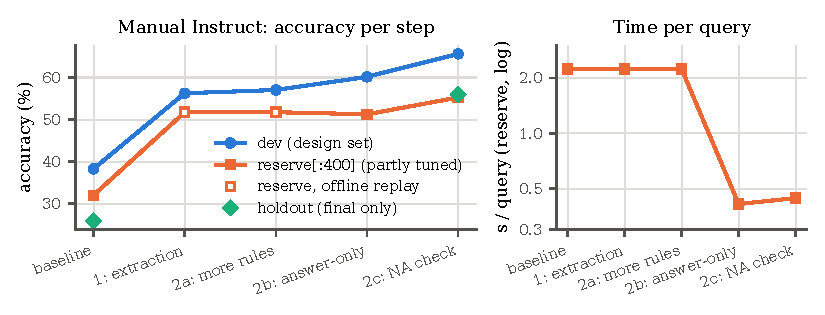
\includegraphics[width=\linewidth]{figures/manual_steps.pdf}
\caption{Manual Instruct optimization, one change per step. Dev is the design set (fitted); reserve[:400] was used
for keep/drop decisions; holdout points are the untouched final evaluations of the baseline and the final manual
version. Open squares are exact offline replays of post-processing on recorded raw outputs.}
\label{fig:manual}
\end{figure}

\paragraph{Evolution.} The Instruct run (12 generations $\times$ 6 children) raised evo accuracy from 54.75\,\% to
62.50\,\% (+31 answers of 400; Figure~\ref{fig:evo}). Two independent lineages reached the same level (62.50 and
62.25\,\%), which suggests a real effect rather than a lucky child. The winning edits added a system prompt that asks
for careful reading of ticks, legends and grids, broadened the ``Not Applicable'' check to lines, intersections and
axes, applied answer cleanup to every answer, and cached processed images. Almost the whole gain is on number-reading
and counting questions (60$\rightarrow$85 of 160 on evo). The Thinking run (2 generations $\times$ 3 children, the
cost of one full evaluation being about an hour) found one improvement: halving the reasoning budget
(1{,}024$\rightarrow$512 tokens), 30\,\% faster on evo at the same accuracy (71.9 vs.\ 74.2\,\% on 128 queries, within
noise).

\begin{figure}[h]
\centering
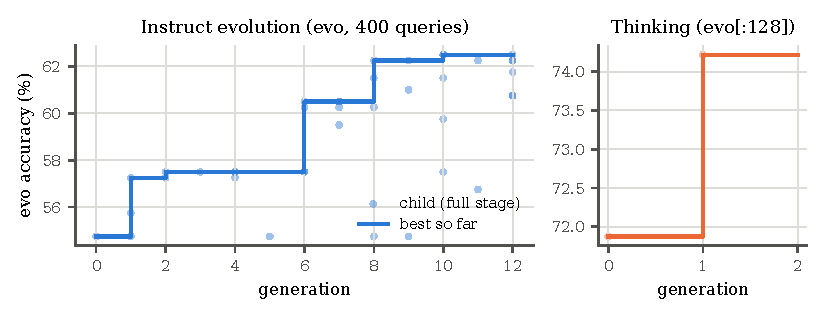
\includegraphics[width=\linewidth]{figures/evolution.pdf}
\caption{Evo accuracy of every child that reached the full stage, and the best so far. These are training numbers;
Table~\ref{tab:holdout} gives the holdout transfer. The Thinking run had only two distinct evaluated children.}
\label{fig:evo}
\end{figure}

\paragraph{Holdout.} Table~\ref{tab:holdout} and Figure~\ref{fig:holdout} compare all versions on the 800 holdout
queries. Instruct evolution transfers: +7.75 points on evo became \textbf{+6.0 on holdout} (56.0$\rightarrow$62.0\,\%;
108 vs.\ 60 discordant answers, $p=0.0003$), again from number-reading and counting questions (132$\rightarrow$174 of
326). Thinking evolution holds up and, with six times more queries than on evo, shows an accuracy gain too:
\textbf{$-$33\,\% time} (28.6$\rightarrow$19.3\,s/query) and \textbf{+2.2 points} (31 vs.\ 13, $p=0.01$). Routing numbers
are composed from the Instruct and Thinking runs (each question answered by the model it is routed to); a direct run
on 32 holdout queries gave identical answers for all 32.

\begin{table}[h]
\centering\small
\caption{Holdout (800 queries, RTX 3090): accuracy, time and correct answers per category (quant = number reading
and counting). The \emph{dev} column is the official 128-query set given with the task (fitted for manual
versions; reproduced with \texttt{bash reproduce.sh}, answer-for-answer identical to the recorded runs).}
\label{tab:holdout}
\begin{tabular}{lrrrrrrrrr}
\toprule
program & dev\,\% & holdout\,\% & s/query & quant & ocr & layout & enum & title & bool \\
 & & & & /326 & /305 & /44 & /34 & /50 & /28 \\
\midrule
naive baseline (Instruct) & 38.3 & 25.9 & 2.61 & 12 & 101 & 25 & 17 & 34 & 13 \\
manual Instruct (\texttt{best\_speed}) & 65.6 & 56.0 & \textbf{0.41} & 132 & 213 & 33 & 17 & 34 & 15 \\
evolved Instruct (\texttt{best\_overall}) & 67.2 & 62.0 & 0.46 & 174 & 210 & 32 & 21 & 37 & 18 \\
manual Thinking & 72.7 & 64.8 & 28.61 & 177 & 232 & 38 & 12 & 34 & 18 \\
evolved Thinking (\texttt{best\_accuracy}) & 74.2 & \textbf{67.0} & 19.27 & 185 & 231 & 38 & 23 & 34 & 18 \\
routing, manual models & 74.2 & 61.6 & 14.45 & 177 & 213 & 33 & 17 & 34 & 15 \\
routing, evolved models & \textbf{75.0} & 63.4 & 8.03 & 185 & 210 & 32 & 21 & 37 & 18 \\
\bottomrule
\end{tabular}
\end{table}

\begin{figure}[h]
\centering
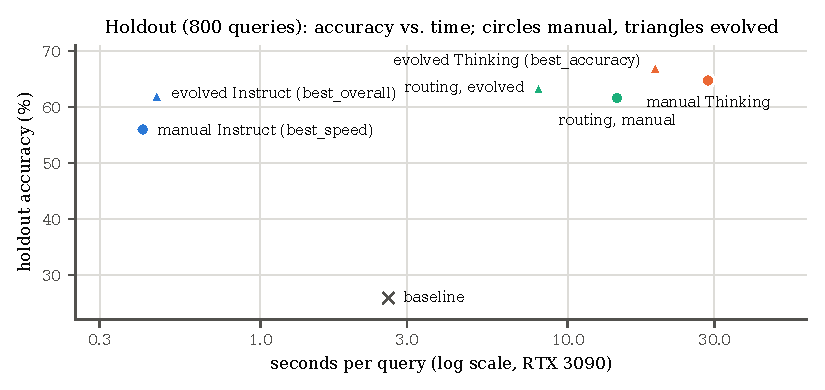
\includegraphics[width=\linewidth]{figures/holdout.pdf}
\caption{Holdout accuracy against time per query. Circles: manual versions; triangles: evolved; the best\_* labels
mark the submitted selections.}
\label{fig:holdout}
\end{figure}

\paragraph{Best accuracy, best speed, best overall.} \texttt{best\_accuracy} and \texttt{best\_speed} were selected on
reserve[800:1000], a slice nothing had used, so that holdout stays an unbiased test of the choice
(Table~\ref{tab:select}). \textbf{Best accuracy} is the evolved Thinking model: 67.0\,\% on holdout, from reasoning
(+53 number-reading answers over manual Instruct), the Instruct prompt engineering it inherits, and the evolved
reasoning budget. \textbf{Best speed} is manual Instruct (0.41\,s/query): the answer-only prompt and 64-token limit
removed the verbose answers that dominated the baseline's time; the rule we fixed beforehand (keep manual Instruct
unless evolved Instruct is $>$10\,\% faster) chose it although the two are within timing noise and evolved Instruct is
4--6 points more accurate. \textbf{Best overall} is evolved Instruct (62.0\,\% at 0.46\,s/query); every more accurate
program is 17--62$\times$ slower, so we decided it on holdout and consider the selection bias negligible.

\begin{table}[h]
\centering\small
\caption{Selection slice reserve[800:1000] (200 queries). Top differences are not significant at this size
(evolved Thinking vs.\ evolved routing: 14 vs.\ 9 discordant answers, $p=0.4$); the ordering agrees with holdout.}
\label{tab:select}
\begin{tabular}{lrr}
\toprule
candidate & accuracy & s/query \\
\midrule
evolved Thinking & \textbf{72.0\,\%} & 14.4 \\
manual Thinking & 71.0\,\% & 21.7 \\
routing, manual models & 70.0\,\% & 9.9 \\
routing, evolved models & 69.5\,\% & 6.5 \\
evolved Instruct & 67.0\,\% & 0.45 \\
manual Instruct & 63.0\,\% & 0.44 \\
\bottomrule
\end{tabular}
\end{table}

\section{Analysis}

\paragraph{The routing reversal.} Thinking answered number-reading and counting questions much better than Instruct
on reserve[:128] and dev, so we routed those question types (recognized from the question template) to Thinking and
the rest to Instruct. On a fresh slice, routing beat Instruct alone by 9.0 points (67.8 vs.\ 58.8\,\%, 49 vs.\ 13
discordant answers, $p<0.001$) and became the pre-registered \texttt{best\_accuracy} candidate. On holdout it still
beats Instruct alone (+5.6 points, $p<10^{-5}$) but \emph{loses to Thinking alone} (61.6 vs.\ 64.8\,\%): Thinking is
also better on OCR-type questions (+19) and layout (+5), which the small design slice had not shown; on dev, too, routing scores at or above Thinking alone (74.2--75.0
vs.\ 72.7--74.2\,\%, Table~\ref{tab:holdout}). \textbf{A design
validated against the wrong baseline can fail on the right one. We caught this only because holdout had been
preserved}; selection then moved to a second fresh slice instead of to holdout. Routing remains a useful middle point
(2$\times$ faster than Thinking alone) but lost its role.

\paragraph{What evolution changed, and what it did not.} Instruct evolution found prompt-level changes that a human
had partly tried (system prompt, ``Not Applicable'' wording) but combined and refined them over 12 generations; the
convergence of two lineages and the holdout transfer support that the gain is real. Thinking evolution chose the
\emph{simplest} suggested mutation, a lower budget. We had measured a stronger one beforehand: cutting recorded
reasoning before its fourth ``Wait'' (the model's second-guessing marker, present in 76\,\% of responses) kept dev
accuracy (93$\rightarrow$93) and raised reserve accuracy (76$\rightarrow$84 of 128) with about 60\,\% fewer reasoning
tokens. The mutation prompt suggested this first, yet four of six children proposed the same budget edit,
byte-identical, despite the ``already tried'' list. LLM-guided evolution at this scale prefers edits that are easy to
express over the most effective ones; a hand-built Wait-stopping version would likely beat what evolution found.

\paragraph{Negative results.} More extraction rules did not help (dev +1, reserve +0): extraction saturates once the
remaining errors are wrong values rather than formatting. The evaluation cascade saved only 10\,\% of Instruct GPU
time net (filters $+28$\,min, early stops $+24$\,min, overhead of the small stages on promoted children $-36$\,min):
a full Instruct evaluation is cheap and 75\,\% of evaluated children passed, so the real saving came from rejecting
duplicates and invalid programs before the GPU. The cascade pays off where a full evaluation is expensive (Thinking:
about 54\,min saved per early stop).

\section{Overfitting audit}
\label{sec:audit}

Holdout is the only split not used for any design decision, and is this report's primary evidence; the one decision
it informed is \texttt{best\_overall}, where the margin makes the bias negligible. Every other number is either fitted
or a single-use check. Dev numbers of the manual versions are fitted: extraction rules, the ``Not Applicable'' wording
and the 64-token limit were derived from dev outputs and gold answers, and the dev$-$reserve gap of manual Instruct grew
from 4.5 to 10.4 points over the steps, a measured sign of fitting. Reserve[:400] became a partial tuning set through
keep/drop decisions; reserve[400:800] and reserve[800:1000] were each used once. Evo numbers are training fitness.
The routing rule is a list of seven substrings copied from CharXiv's question templates (its source code, not its
answers); a check that it misroutes none of the 4{,}000 validation questions only verifies the string matching
against those templates, not generalization. The routing rule and the choice of routed types are a manual design and
were never a mutation target.

\section{Limitations and future work}

The evolution runs are small (72 and 6 children), limited by GPU time per evaluation; the Thinking run had only two
distinct evaluated children. The mutation models often repeated ideas, and Instruct's promotion margin let neutral
edits pay for a full evaluation. A hidden test set may differ from our holdout in difficulty (the naive baseline scores
38.3\,\% on dev but 25.9\,\% on holdout). Future work: asynchronous evaluation on several GPUs; rejecting a reply whose
idea matches a tried one before applying it; a reasoning-stopping criterion inside generation (the measured Wait
cut); speed work we deliberately deferred (fast image processor, compiled decoding, vLLM; the Thinking model runs at
about 25\,\% GPU utilization because of per-token Python overhead); and meta-prompt evolution.

\begin{thebibliography}{9}
\bibitem[Novikov et~al.(2025)]{alphaevolve} A.~Novikov et~al. AlphaEvolve: A coding agent for scientific and
algorithmic discovery. Google DeepMind, 2025.
\bibitem[Wang et~al.(2024)]{charxiv} Z.~Wang et~al. CharXiv: Charting gaps in realistic chart understanding in
multimodal LLMs. NeurIPS Datasets and Benchmarks, 2024.
\bibitem[Qwen Team(2025)]{qwen3vl} Qwen Team. Qwen3-VL technical report. 2025.
\bibitem[Mouret and Clune(2015)]{mapelites} J.-B.~Mouret and J.~Clune. Illuminating search spaces by mapping elites.
arXiv:1504.04909, 2015.
\bibitem[McNemar(1947)]{mcnemar} Q.~McNemar. Note on the sampling error of the difference between correlated
proportions or percentages. Psychometrika 12(2):153--157, 1947.
\end{thebibliography}

\end{document}
